\documentclass[12pt,a4]{article}







\usepackage{graphicx,amsmath,amssymb,amsthm, boxedminipage,xcolor}

%\usepackage[lined,boxed]{algorithm2e}

\usepackage{algorithm}
\usepackage{algpseudocode}

%\usepackage{algorithmic}
\usepackage{algpseudocode}
\usepackage{amsmath}
\usepackage{graphics}
\usepackage{epsfig}

\newtheorem{theorem}{Theorem}[section]
\newtheorem{proposition}[theorem]{Proposition}
\newtheorem{lemma}[theorem]{Lemma}
\newtheorem{corollary}[theorem]{Corollary}
\newtheorem{definition}[theorem]{Definition}

\newtheorem*{theorem*}{Theorem}
\newtheorem*{lemma*}{Lemma}
\newtheorem*{proposition*}{Proposition}


\newtheorem{exercise}[theorem]{Exercise}
\newtheorem{exerciseD}[theorem]{*Exercise}
\newtheorem{exerciseDD}[theorem]{**Exercise}

\let\oldexercise\exercise
\renewcommand{\exercise}{\oldexercise\normalfont}

%\let\oldexerciseD\exerciseD
%\renewcommand{\exerciseD}{\oldexerciseD\normalfont}

%\let\oldexerciseDD\exerciseDD
%\renewcommand{\exerciseDD}{\oldexerciseDD\normalfont}

\newcommand{\E}{\mathbb{E}}
%\newcommand{\nth}[1]{#1^{\textsuperscript{th}}}
\newcommand{\scalar}[2]{\ensuremath{\langle #1, #2\rangle}}
\newcommand{\floor}[1]{\left\lfloor #1 \right\rfloor}
\newcommand{\ceil}[1]{\left\lceil #1 \right\rceil}
\newcommand{\norm}[1]{\|#1\|}
\newcommand{\pfrac}[2]{\left(\frac{#1}{#2}\right)}
\newcommand{\nth}[1]{#1^{\textsuperscript{th}}}
\newcommand{\core}{\textnormal{core}}



\newif\ifsolution

\solutionfalse

\newcommand{\answer}[1]{
\ifsolution
{\color{blue} #1}
\else
\fi
}



\newcommand{\poly}{\textnormal{poly}}
\newcommand{\quasipol}{\textnormal{quasipol}}
\newcommand{\ssubexp}{\textnormal{stronglySubExp}}
\newcommand{\wsubexp}{\textnormal{weaklySubExp}}
\newcommand{\simplyexp}{\textnormal{E}}
\newcommand{\expo}{\textnormal{Exp}}



\newcommand{\N}{\mathbb{N}}
\newcommand{\nn}{\mathbb{N}_0^n}
\newcommand{\R}{\mathbb{R}}
\newcommand{\Z}{\mathbb{Z}}


\definecolor{darkgreen}{rgb}{0,0.6,0}


\date{}

\title{
  Mathematical Foundations \\of \\Computer Science\\
  \vspace{3mm}
{\normalsize CS 499,	Shanghai Jiaotong University,  Dominik Scheder}
}

\begin{document}

\maketitle

%\begin{quotation}
%  You are welcome to discuss the exercises in the discussion
%  forum. Please take them serious. Doing the exercises is as important
%  than watching the videos.
%
%  I intentionally included very challenging exercises and marked them
%  with one or two ``$*$''. No star means you should be able to solve
%  the exercises without big problems once you have understood
%  the material from the video lecture. One star means it requires 
%  significant additional thinking. Two stars means it is not 
%  unlikely that you will fail to solve them, even once you have understood
%  the material and thought a lot about the exercise. Don't feel bad
%  if you fail. Failure is part of learning.
%
%  This is the first time this course is online. Thus there might be mistakes
%  (typos or more serious conceptual mistakes) in the exercises. I will be 
%  grateful if you point them out to me!
%\end{quotation}




\setcounter{section}{1}


\begin{itemize}
 \item Homework assignment published on Monday, 2018-03-05.
 \item Work on it and submit a first solution or questions by Sunday, 2018-03-11, 12:00 by
 email to me and the TAs.
 \item You will receive feedback by Wednesday, 2018-03-14.
 \item Submit your final solution by Sunday, 2018-03-18 to me and the TAs.
\end{itemize}



\section{Partial Orderings}



\subsection{Equivalence Relations as a Partial Ordering}

An equivalence relation $R \subseteq V \times V$ is basically the same as a partition
of $V$. A {\em partition} of $V$ is a set $\{V_1,\dots,V_k\}$ where
(1) $V_1 \cup \dots \cup V_k = V$ and (2) the $V_i$ are pairwise disjoint,
i.e., $V_i \cap V_j  = \emptyset$ for $1 \leq i < j \leq k$. For example,
$\{ \{1\}, \{2,3\}, \{4\} \}$ is a partition of $\{1,2,3,4\}$ but
$\{ \{1\}, \{2,3\}, \{1,4\}\}$ is not.



\begin{exercise}
  Let $E_4$ be the set of all equivalence relations on $\{1,2,3,4\}$. Note that
  $E_4$ is ordered by set inclusion, i.e.,
  \begin{align*}
     (E_4, \{ (R_1,R_2) \in E_4 \times E_4 \ | \ R_1 \subseteq R_2 \} )
  \end{align*}
  is a partial ordering.
  \begin{enumerate}
    \item Draw the Hasse diagram of this partial ordering in a  nice way.

    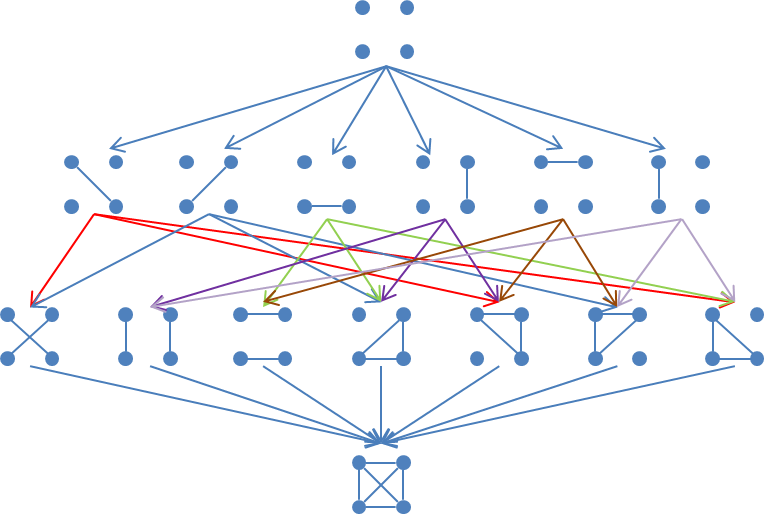
\includegraphics[width = 0.8 \textwidth]{hasse.png}
    \item What is the size of the largest chain?
    
    4.
    \item What is the size of the largest antichain? 
    
    7.
  \end{enumerate}
  \end{exercise}


\subsection{Chains and Antichains}

Define the partially ordered set $(\nn, \leq)$ as follows:
$x \leq y$ if $x_i \leq y_i$ for all $1 \leq i \leq n$. For example,
$(2,5,4) \leq (2,6,6)$ but $(2,5,4) \not \leq (3,1,1)$.

\begin{exercise}
  Consider the infinite partially ordered set $(\nn, \leq)$.
  \begin{enumerate}
  \item
    Which elements are minimal? Which are maximal?
    \par The minimal element is $(0,0,0,\cdots,0)$.(There are $n 0$s in the element.)
    \par No element is maximal.
  \item Is there a minimum? A maximum?
    \par The minimum element is $(0,0,0,\cdots,0)$.(There are $n 0$s in the element.)
    \par No element is maximum.
  \item Does it have an infinite chain?
    \par Yes.
    \par There is an example: $\{(0,0,0,\cdots,0),(1,0,0,\cdots,0),(1,1,0,\cdots,0),\cdots,(1,1,1,\cdots,1)\}$
  \item Does it have arbitrarily large antichains? That is, can you find an
  antichain $A$ of size $|A| = k$ for every $k \in \N$?
    \par Yes. We consider an antichain like this:
    \begin{center}
    $\{(1,0,0,\cdots,0),(0,1,0,\cdots,0),
    (0,0,1,\cdots,0),\cdots,(0,0,0,\cdots,1)\}$
    \end{center}
    For the $k^{th}$ element, there is only one $1$ in the $k^{th}$ position, and other positions are all occupied by $0$. And the antichain consists of these $k$ elements.
\end{enumerate}
\end{exercise}

\begin{exerciseD}
  Does every infinite subset $S \subseteq \nn$ contain
  an infinite chain?
\end{exerciseD}

\begin{proof}
\par
Base case $n=1$: Apparently, every two elements in set $N_0^0$ is comparable since there is only one dimension. If there exists an infinite subset $S \subseteq \N_0^0$, the subset $S$ itself is an infinite chain.
So, the theorem holds when $n=1$. \\
Inductive hypothesis: \\
\indent Suppose the theorem holds for all values of $n$ up to some $k$, $k \geq 1$.\\
Inductive step: \\
\indent Let $n=k+1$. If there exists an infinite subset $S \subseteq \N_0^{k+1}$, note
\begin{equation}
\begin{aligned}
S_1 &= \{ (a_1, a_2, ..., a_k) &| (a_1, a_2, ..., a_k, a_{k+1}) \in S \}\\
S_2 &= \{ a_{k+1} &| (a_1, a_2, ..., a_k, a_{k+1}) \in S \}
\end{aligned}
\end{equation}
\indent Since $S$ is infinite, at least one of $S_1, S_2$ is infinite. \\
\indent Suppose $S_1$ is infinite, according to inductive hypothesis, there is an infinite chain $C_k$ for $S_1 \subseteq \N_0^k$.
\begin{equation}
\begin{aligned}
C_k &= (A_1, A_2, \cdots), A_1 \leq A_2 \leq \cdots \\
A_i &= (a_{i1}, a_{i2}, \cdots, a_{ik})
\end{aligned}
\end{equation}
\indent Now we construct an infinite chain $C_{k+1}$ for $S \subseteq \N_0^{k+1}$.  Take $b \in S_2$, we append every $A_i$ with $b$ to get $B_i$.
\begin{equation}
\begin{aligned}
B_i &= (a_{i1}, a_{i2}, \cdots, a_{ik}, b)\\
C_{k+1} &= (B_1, B_2, \cdots), B_1 \leq B_2 \leq \cdots
\end{aligned}
\end{equation}
\indent So $C_{k+1}$ is an infinite chain for $S \subseteq \N_0^{k+1}$.\\
\indent Now suppose $S_1$ is finite and $S_2$ is infinite. Notice that $S_2$ itself is an infinite chain. We take $(a_1, a_2, ..., a_k) \in S_1$ and we can construct an infinite chain for $S \subseteq \N_0^{k+1}$ in a similar way.

So, the theorem holds for $n=k+1$.
By the principle of mathematical induction, the theorem holds for all $n \in \mathbb{N}$.
\end{proof}

\begin{exercise}
  Show that $(\nn,\leq)$ has no infinite antichain. \textbf{Hint.} Use
  the previous exercise.
\end{exercise}
\begin{proof}
We proof it by contradiction. Suppose there is an infinite antichain which is also a subset of $\nn$. But from Exercise 2.3, it is clear to us that every infinite subset $S \subseteq \nn$ contain an infinite chain. So there is a contradiction. Consequently, $(\nn,\leq)$ has no infinite antichain.
\end{proof}



Consider the induced ordering on $\{0,1\}^n$. That is, for $x,y\in \{0,1\}^n$
we have $x \leq y$ if $x_i \leq y_i$ for every coordinate $i \in [n]$.

\begin{exercise}
 Draw the Hasse diagrams of $(\{0,1\}^n, \leq)$ for $n=2,3$.

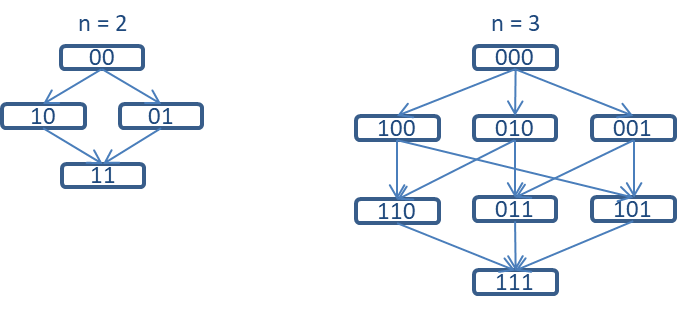
\includegraphics[width = 0.8 \textwidth]{23.jpg}
\end{exercise}

\begin{exercise}
  Determine the maximum, minimum, maximal, and minimal elements of
  $\{0,1\}^n$.
\end{exercise}
\begin{center}
Maximum element:$(1,1,1,\cdots,1)$
\par Maximal element:$(1,1,1,\cdots,1)$
\par Minimum element:$(0,0,0,\cdots,0)$
\par Minimal element:$(0,0,0,\cdots,0)$
\end{center}
\begin{exercise}
  What is the longest chain of $\{0,1\}^n$?
  \par One of the examples is as follows:
  \begin{center}
  $\{(0,0,0,\cdots,0),(1,0,0,\cdots,0),
  (1,1,0,\cdots,0),\cdots,(1,1,1,\cdots,1)\}$
  \end{center}
\end{exercise}


\begin{exerciseDD}
  What is the largest antichain of $\{0,1\}^n$?
\end{exerciseDD}



\subsection{Infinite Sets}

In the lecture (and the lecture notes) we have showed that $\N \times \N \cong \N$, i.e.,
there is a bijection $f: \N \times \N \rightarrow \N$. From this, and by induction, it follows
quite easily that $\N^k \cong \N$ for every $k$.

\begin{exercise}
  Consider $\mathbb{N}^*$, the set of all finite sequences of natural numbers, that is, $\mathbb{N}^{*}=\{\epsilon\}\cup\mathbb{N}\cup\mathbb{N}^2\cup\mathbb{N}^3\ldots$. Here,$\epsilon$ is the empty sequence. Show that $\mathbb{N}\cong\mathbb{N}^*$ by defining a bijection $\mathbb{N}\to\mathbb{N}^*$.
\end{exercise}

\begin{proof}
First we can proof $\{0,1\}^*\cong\mathbb{N}$:\\
Formally, we can define a function:
\begin{align}
\nonumber f_1:\{0,1\}^*\to\mathbb{N},&\forall a=(a_1^{(n)},a_2^{(n)},a_3^{(n)},\ldots,a_n^{(n)}) \in \{0,1\}^{*},a_i^{(n)}=0 or 1,i=1,2,\ldots,n \\
\nonumber &\to 10^n+\sum_{i=1}^n10^{i-1}a_i^{(n)}
\end{align}
\[\]
For example:$f_1(001010)=1001010_{10}$.\\Then we can define another function:
\[f_2:\mathbb{N}\to\{0,1\}^*,decimal \quad number \to binary\]
For example:$f_2(16)=10000$.So we get the conclusion:\\
\[\{0,1\}^*\cong\mathbb{N} \eqno(1)\]
Secondly, we can proof $\{0,1\}^*\cong\mathbb{N}^*$:\\
Define a function:
\[f_3:\{0,1\}^*\to\mathbb{N}^*,x \to x\]
Another function:
\begin{align}
\nonumber f_4:\mathbb{N}^*\to\{0,1\}^*,&\forall a=(a_1^{(n)},a_2^{(n)},a_3^{(n)},\ldots,a_n^{(n)}) \in \mathbb{N}^{*},a_i^{(n)} \in \mathbb{N},i=1,2,\ldots,n\\
\nonumber \to&(a_1^{(n)}\%2,a_2^{(n)}\%2,a_3^{(n)}\%2,\ldots,a_n^{(n)}\%2),i=1,2,\ldots,n
\end{align}
For example, $f_4((154,3,89,23,48))=01110$. So we get the conclusion:\\
\[\{0,1\}^*\cong\mathbb{N}^*\eqno(2)\]
According (1) and (2), $\mathbb{N}\cong\mathbb{N}^*$ is obvious.
\end{proof}

\begin{exercise}
   Show that $R \cong R \times R$. \textbf{Hint:} Use the fact that
   $R \cong \{0,1\}^{\N}$ and thus show that $\{0,1\}^{\N} \cong \{0,1\}^{\N} \times \{0,1\}^{\N}$.
\end{exercise}

\begin{proof}
Obvious, there exits a function:
\begin{align}
\nonumber f_1:\{0,1\}^{\mathbb{N}} \to \{0,1\}^{\mathbb{N}} \times \{0,1\}^{\mathbb{N}}, x \to (x, 0000\ldots)
\end{align}
Then, we define a function:
\begin{align}
\nonumber f_2:\{0,1\}^{\mathbb{N}} \times \{0,1\}^{\mathbb{N}} \to \{0,1\}^{\mathbb{N}}, (a_1a_2a_3\ldots, b_1b_2b_3\ldots) \to (a_1b_1a_2b_2a_3b_3\ldots)
\end{align}
Such as:\\
\begin{center}
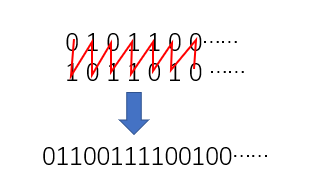
\includegraphics[scale=0.8]{1.png} 
\end{center}
Therefore, we proof $\{0,1\}^{\mathbb{N}} \cong \{0,1\}^{\mathbb{N}} \times \{0,1\}^{\mathbb{N}}$, and then $R \cong R \times R$.
\end{proof}

\begin{exercise}
Consider $R^{\mathbb{N}}$, the set of all infinite sequences $(r_1, r_2, r_3, \ldots)$ of real numbers. Show that $R \cong R^{\mathbb{N}}$. \textbf{Hint:} Again, use the fact that $R \cong \{0,1\}^{\mathbb{N}}$.
\end{exercise}

\begin{proof}
We only need to proof that ${(\{0,1\}^{\mathbb{N}})}^{\mathbb{N}} \cong \{0,1\}^{\mathbb{N}}$.
Firstly, we can know the following function easily:
\begin{align}
f_1:\{0,1\}^{\mathbb{N}} \to {(\{0,1\}^{\mathbb{N}})}^{\mathbb{N}}, x \to (x, 00000\ldots, 00000\ldots,00000\ldots, \ldots).
\end{align}
\begin{center}
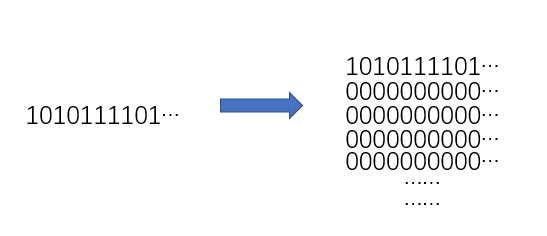
\includegraphics[scale=0.6]{2.png} 
\end{center}
Then,define a complexer function:
\begin{align}
f_2:{(\{0,1\}^{\mathbb{N}})}^{\mathbb{N}} \to \{0,1\}^{\mathbb{N}},(x_1^1x_2^1x_3^1\ldots,x_1^2x_2^2x_3^2\ldots,x_1^3x_2^3x_3^3\ldots
,\ldots) \to (x_1^1x_1^2x_2^2x_1^2x_1^3x_2^3\ldots),x_i^j=0\:or\:1
\end{align}
\begin{center}
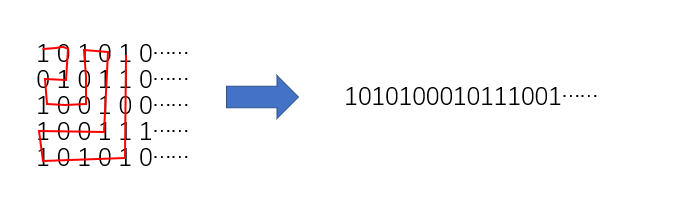
\includegraphics[scale=0.6]{3.png} 
\end{center}
Now, we can infer ${(\{0,1\}^{\mathbb{N}})}^{\mathbb{N}} \cong \{0,1\}^{\mathbb{N}}$ is true. Thus, $R \cong R^{\mathbb{N}}$.
\end{proof}

Next, let us view $\{0,1\}^{\N}$ as a partial ordering: given two elements $\mathbf{a}, \mathbf{b} \in \{0,1\}^{\N}$,
that is, sequences $\mathbf{a} = (a_1,a_2,\dots)$ and $\mathbf{b} = (b_1,b_2,\dots)$, we define
$\mathbf{a} \leq \mathbf{b}$ if $a_i \leq b_i$ for all $i \in \N$. Clearly,
$(0,0,\dots)$ is the minimum element in this ordering and $(1,1,\dots)$ the maximum.\\

\begin{exercise}
   Give a countably infinite chain in $\{0,1\}^{\N}$. Remember that a set $A$ is countably infinite
   if $A \cong \N$.
\end{exercise}
    $$ (0, 0, 0, \dots) $$
    $$ (1, 0, 0, \dots) $$
    $$ (1, 1, 0, \dots) $$
    $$ (1, 1, 1, \dots) $$
    $$ \dots $$

    Since there are countably infinite bits in every element, we can construct countably infinite chain in $\{0,1\}^{\N}$ as showed above.

\begin{exercise}
   Find a countably infinite antichain in $\{0,1\}^{\N}$.
\end{exercise}
    $$ (1, 0, 0, \dots) $$
    $$ (0, 1, 0, \dots) $$
    $$ (0, 0, 1, \dots) $$
    $$ \dots $$

    Since there are countably infinite bits in every element, we can construct countably infinite chain in $\{0,1\}^{\N}$ as showed above.


\begin{exercise}
   Find an uncountable antichain in $\{0,1\}^{\N}$. That is, an antichain $A$ with $A \cong \R$.
\end{exercise}
    Since $\{0,1\}^{\N} \cong \R$, there is a bijection: $x \leftrightarrow \mathbf{t}$, $x \in \R, \mathbf{t} \in \{0,1\}^{\N}$. Let's consider $\mathbf{t_i}$.
    $$ \mathbf{t_i} = (a_1, a_2, \dots), a_k \in \{0,1\}, k \in \N $$
    Define $\bar{\mathbf{t_i}} = (1-a_1, 1-a_2, \dots)$.
    Then construct $\hat{\mathbf{t_i}}$ as:
    $$ \hat{\mathbf{t_i}} = (a_1, 1-a_1, a_2, 1-a_2, \dots) $$
    Consider $\hat{\mathbf{t_i}}, \hat{\mathbf{t_j}}, \forall i, j \in \N, i \neq j$.

    \textbf{Case 1:} If $\mathbf{t_i} \nleq \mathbf{t_j}$, obviously, $\hat{\mathbf{t_i}} \nleq \hat{\mathbf{t_j}}$.

    \textbf{Case 2:} If $\mathbf{t_i} \leq \mathbf{t_j}$
    
    $$\mathbf{t_i}=(a_1, a_2, \dots)\quad \bar{\mathbf{t_i}}=(1-a_1, 1-a_2, \dots)$$
    $$\mathbf{t_j} = (b_1, b_2, \dots)\quad \bar{\mathbf{t_j}} = (1-b_1, 1-b_2, \dots)$$

    According to the definition of $\mathbf{a} \leq \mathbf{b}$, we know that $a_k \leq b_k$. So, $\bar{\mathbf{t_i}} \geq \bar{\mathbf{t_j}}$.

    Compare every bit of $\hat{\mathbf{t}}$.
    $$
    \begin{array}{c|lcccr}
    \hat{\mathbf{t}} & 1 & 2 & 3 & 4 & \dots \\
    \hline
    \hat{\mathbf{t_i}} & a_1 & 1-a_1 & a_2 & 1-a_2 & \dots \\
    \hat{\mathbf{t_j}} & b_1 & 1-b_1 & b_2 & 1-b_2 & \dots \\
    \end{array}
    $$

    Since $a_k \leq b_k$, $1-a_k \geq 1-b_k$. 
    
    And since $i \neq j$, $\mathbf{t_i}, \mathbf{t_j}$ are not the same $\mathbf{t}$, which means that $\exists \eta, a_{\eta} < b_{\eta}, 1-a_{\eta} > 1-b_{\eta}$. So, $\hat{\mathbf{t_i}} \nleq \hat{\mathbf{t_j}}$.

    Therefore, $\hat{\mathbf{t_1}} \quad \hat{\mathbf{t_2}} \quad \dots$ is an uncountable antichain in $\{0,1\}^{\N}$.


\begin{exerciseDD}
   Find an uncountable chain in $\{0,1\}^{\N}$. That is, an antichain $A$ with $A \cong \R$.
\end{exerciseDD}

\textbf{Question:} 

\begin{enumerate}
    \item We are wondering if there is an easier or another way to solve 2.14.
    \item We are wondering how to illustrate the obvious conclusion in 2.8.
    
\end{enumerate}

\end{document}



